\section{Kategorie dokładne Quillena i kategorie egzaktne Barra}\label{cat:sec:exact-quillen-barr}

Pojęcie dokładności występuje w teorii kategorii w dwóch odmiennych znaczeniach. Struktura dokładna Quillena na kategorii addytywnej wyróżnia pewne pary jądro--kojądro, które odgrywają rolę krótkich ciągów dokładnych. Nie wymaga istnienia wszystkich jąder ani kojąder. Z kolei dokładność w sensie Barra dotyczy kategorii regularnych, w których każda wewnętrzna relacja równoważności pochodzi od iloczynu włóknistego pewnego morfizmu z samym sobą. To drugie pojęcie nie wymaga addytywności. Rozróżnienie jest istotne: kategorie grup i zbiorów są egzaktne w sensie Barra, a nie są kategoriami addytywnymi.

Korzystamy z pojęć kategorii addytywnej i abelowej z rozdziału~\ref{cat:sec:abelian-categories} oraz ze zmiany bazy i sum amalgamowanych z rozdziału~\ref{sec:equalizatory}. Wszystkie kategorie rozpatrujemy jako lokalnie małe w ustalonym uniwersum.

\subsection{Struktury dokładne Quillena}

\begin{definicja}[Para jądro--kojądro]\label{cat:def:exact-kernel-cokernel}
W kategorii addytywnej $\mathcal E$ parę morfizmów
\[
 A\xrightarrow{i}B\xrightarrow{p}C
\]
nazywamy parą jądro--kojądro, jeśli $i$ jest jądrem $p$, a $p$ jest kojądrem $i$ w sensie definicji~\ref{cat:def:kernel-cokernel}. W szczególności $pi=0$, $i$ jest monomorfizmem, a $p$ epimorfizmem.
\end{definicja}

Nie zakładamy, że każda para morfizmów z zerowym złożeniem jest parą jądro--kojądro. W kategorii abelowej powyższy warunek odpowiada dokładności ciągu $0\to A\to B\to C\to0$, na mocy stwierdzenia~\ref{cat:prop:ses-kernel-cokernel}.

\begin{definicja}[Kategoria dokładna Quillena]\label{cat:def:quillen-exact}
Struktura dokładna $\mathscr E$ na kategorii addytywnej $\mathcal E$ jest klasą par jądro--kojądro, zamkniętą na izomorfizmy diagramów i spełniającą następujące aksjomaty. Pary należące do $\mathscr E$ nazywamy konflacjami (wyróżnionymi krótkimi ciągami dokładnymi), ich pierwsze morfizmy inflacjami, a drugie deflacjami. Zapisujemy je jako
\[
 A\overset{i}{\lhook\joinrel\longrightarrow}B
 \overset{p}{\twoheadrightarrow}C.
\]
\begin{enumerate}
 \item[(E0)] Identyczność obiektu zerowego jest inflacją i deflacją.
 \item[(E1)] Złożenie dwóch inflacji jest inflacją; złożenie dwóch deflacji jest deflacją.
 \item[(E2)] Dla deflacji $p:B\to C$ i dowolnego $f:C'\to C$ istnieje iloczyn włóknisty $B'\to C'$ morfizmu $p$ wzdłuż $f$, a indukowany morfizm $p':B'\to C'$ jest deflacją.
 \item[(E2$^{\mathrm{op}}$)] Dla inflacji $i:A\to B$ i dowolnego $g:A\to A'$ istnieje suma amalgamowana $B'$ morfizmów $i,g$, a indukowany morfizm $i':A'\to B'$ jest inflacją.
\end{enumerate}
Parę $(\mathcal E,\mathscr E)$ nazywamy kategorią dokładną.
\end{definicja}

Strzałka z haczykiem lub podwójnym grotem w tym rozdziale, gdy mowa o strukturze Quillena, oznacza morfizm dopuszczalny w wybranej strukturze, a nie dowolny monomorfizm lub epimorfizm. Pojęcie konflacji określa więc dodatkowe dane na kategorii addytywnej.

\begin{center}
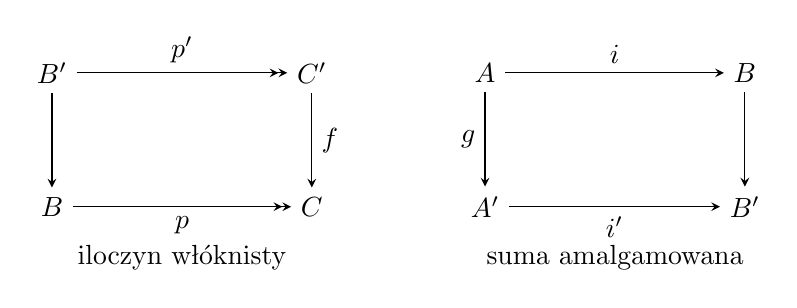
\begin{tikzpicture}[>=stealth]
 \node (b1) at (0,1.7) {$B'$};
 \node (c1) at (3.3,1.7) {$C'$};
 \node (b) at (0,0) {$B$};
 \node (c) at (3.3,0) {$C$};
 \draw[->>] (b1)--node[above] {$p'$}(c1);
 \draw[->] (b1)--(b);
 \draw[->] (c1)--node[right] {$f$}(c);
 \draw[->>] (b)--node[below] {$p$}(c);
 \node at (1.65,-0.65) {iloczyn włóknisty};
 \node (a) at (5.5,1.7) {$A$};
 \node (d) at (8.8,1.7) {$B$};
 \node (a1) at (5.5,0) {$A'$};
 \node (d1) at (8.8,0) {$B'$};
 \draw[->] (a)--node[above] {$i$}(d);
 \draw[->] (a)--node[left] {$g$}(a1);
 \draw[->] (d)--(d1);
 \draw[->] (a1)--node[below] {$i'$}(d1);
 \node at (7.15,-0.65) {suma amalgamowana};
\end{tikzpicture}
\end{center}

Aksjomaty są symetryczne względem przejścia do kategorii przeciwnej: zamiana kierunków wszystkich strzałek zamienia jądra na kojądra, inflacje na deflacje oraz iloczyny włókniste na sumy amalgamowane. Dlatego w dalszych dowodach wskazujemy argument dla jednego rodzaju morfizmów i, o ile nie ma dodatkowych niesymetrycznych założeń, stosujemy go w kategorii przeciwnej.

\begin{stwierdzenie}[Rozkładalne pary w każdej strukturze dokładnej]\label{cat:prop:quillen-split-included}
W każdej kategorii dokładnej wszystkie pary izomorficzne z
\[
 A\xrightarrow{\binom{\id_A}{0}} A\oplus C
 \xrightarrow{(0,\id_C)}C
\]
są konflacjami. W szczególności wszystkie izomorfizmy są zarazem inflacjami i deflacjami.
\end{stwierdzenie}
\begin{proof}
Iloczyn włóknisty deflacji $\id_0:0\to0$ wzdłuż $X\to0$ jest dany przez $X$ z projekcją $\id_X:X\to X$ oraz jedynym morfizmem $X\to0$. Stąd (E2) daje deflację $\id_X$. Jej jądrem jest $0\to X$, zatem para $0\to X\xrightarrow{\id_X}X$ jest konflacją: jądro w dowolnej konflacji kończącej się $\id_X$ jest izomorficzne z $0\to X$. Z argumentu przeciwnego dostajemy konflację $X\xrightarrow{\id_X}X\to0$, w szczególności deflację $X\to0$.

Iloczyn włóknisty deflacji $A\to0$ wzdłuż $C\to0$ to produkt $A\oplus C$ z projekcją na $C$. Aksjomat (E2) daje deflację $(0,\id_C)$. Jej jądrem jest standardowa inkluzja $A\to A\oplus C$: morfizm z $Z$ do biproduktu, którego druga współrzędna jest zerowa, faktoryzuje się jednoznacznie przez pierwszą inkluzję. Zamknięcie na izomorfizmy par daje więc żądaną konflację. Każdy izomorfizm $X\to Y$ jest izomorficzny jako strzałka z $\id_X$, będącą zarówno inflacją, jak i deflacją; odpowiednie pary są konflacjami po przeniesieniu przez ten izomorfizm.
\end{proof}

\subsection{Przykłady struktur dokładnych}

\begin{twierdzenie}[Struktura rozkładalna]\label{cat:thm:quillen-split-structure}
Na każdej kategorii addytywnej istnieje struktura dokładna $\mathscr E_{\mathrm{sp}}$ złożona z par izomorficznych z rozkładalnymi parami z poprzedniego stwierdzenia. Jest to najmniejsza struktura dokładna względem inkluzji klas konflacji.
\end{twierdzenie}
\begin{proof}
Standardowe pary są parami jądro--kojądro przez własność uniwersalną biproduktu: morfizm zerujący pierwszą inkluzję ma jedyną faktoryzację przez drugą projekcję, a dualna własność daje jądro. Klasa jest z definicji zamknięta na izomorfizmy i zawiera parę obiektów zerowych z morfizmami $\id_0$.

Jeżeli $p:B\to C$ oraz $q:C\to D$ są deflacjami rozkładalnymi, to istnieją izomorfizmy $B\cong K\oplus C$ i $C\cong L\oplus D$ przenoszące je na odpowiednie projekcje. Ich złożenie identyfikuje $B$ z $(K\oplus L)\oplus D$ i $qp$ z projekcją na $D$. Jest zatem deflacją rozkładalną. Argument w kategorii przeciwnej dowodzi analogicznego warunku dla inflacji.

Aby sprawdzić (E2), wystarczy rozpatrzyć projekcję $p:K\oplus C\to C$ i morfizm $f:C'\to C$. Iloczyn włóknisty to $K\oplus C'$ z projekcją na $C'$ i morfizmem $\id_K\oplus f:K\oplus C'\to K\oplus C$. Istotnie, dla morfizmów $u:Z\to K\oplus C$ oraz $v:Z\to C'$ spełniających $pu=fv$ jedynym morfizmem do proponowanego iloczynu jest $\langle p_Ku,v\rangle$, gdzie $p_K$ jest pierwszą projekcją. Obie współrzędne są wymuszone przez warunki iloczynu włóknistego. Nowa projekcja jest deflacją rozkładalną. Przez przejście do kategorii przeciwnej otrzymujemy (E2$^{\mathrm{op}}$). Wszystkie aksjomaty zachodzą, a minimalność wynika ze stwierdzenia~\ref{cat:prop:quillen-split-included}.
\end{proof}

\begin{twierdzenie}[Struktura abelowa i podkategorie zamknięte na rozszerzenia]\label{cat:thm:quillen-extension-closed}
Niech $\mathcal A$ będzie kategorią abelową, a $\mathcal E$ jej pełną podkategorią addytywną, zamkniętą na izomorfizmy w $\mathcal A$ i na rozszerzenia: gdy $0\to A\to B\to C\to0$ jest dokładny w $\mathcal A$ oraz $A,C\in\mathcal E$, to $B\in\mathcal E$. Pary morfizmów w $\mathcal E$, które są krótkimi ciągami dokładnymi w $\mathcal A$, tworzą strukturę dokładną na $\mathcal E$.
\end{twierdzenie}
\begin{proof}
Pełność $\mathcal E$ zapewnia, że uniwersalne własności jądra i kojądra pary w $\mathcal A$ pozostają prawdziwe po ograniczeniu obiektów testujących do $\mathcal E$. Zamknięcie na izomorfizmy oraz (E0) są spełnione.

Dla dwóch deflacji $p:B\to C$ oraz $q:C\to D$ w $\mathcal E$ ich jądra $K_p,K_q$ należą do $\mathcal E$. Złożenie $qp$ jest epimorfizmem w $\mathcal A$. Jądro $K$ złożenia jest iloczynem włóknistym $p$ i inkluzji $K_q\to C$: morfizm $Z\to B$ zerowany przez $qp$ ma obraz po złożeniu z $p$ faktoryzujący się jednoznacznie przez $K_q$. Z uniwersalnej własności tego iloczynu otrzymujemy morfizm $K\to K_q$; jest on epimorfizmem przez stabilność epimorfizmów przy zmianie bazy w kategorii abelowej (twierdzenie~\ref{cat:thm:abelian-base-change}). Jego jądrem jest $K_p$: morfizm do $K$ zerowany przez projekcję do $K_q$ jest dokładnie morfizmem do $B$ zerowanym przez $p$, z odpowiednią faktoryzacją. Mamy więc krótki ciąg dokładny
\[
 0\longrightarrow K_p\longrightarrow K\longrightarrow K_q\longrightarrow0.
\]
Z zamknięcia na rozszerzenia $K\in\mathcal E$, stąd $qp$ jest deflacją. Kategoria przeciwna do $\mathcal A$ jest abelowa, a warunek zamknięcia na rozszerzenia jest niezmienniczy względem zmiany kierunku strzałek; argument ten daje również składanie inflacji.

Dla deflacji $p:B\to C$ oraz $f:C'\to C$ w $\mathcal E$ bierzemy iloczyn włóknisty w $\mathcal A$. Twierdzenie~\ref{cat:thm:abelian-base-change} daje krótki ciąg dokładny $0\to K_p\to B'\xrightarrow{p'}C'\to0$. Zatem $B'\in\mathcal E$ i $p'$ jest deflacją. Iloczyn pozostaje iloczynem włóknistym w pełnej podkategorii, co dowodzi (E2). Przechodząc do kategorii przeciwnej, otrzymujemy (E2$^{\mathrm{op}}$).
\end{proof}

\begin{przyklad}[Kategorie abelowe]\label{cat:ex:quillen-abelian}
Biorąc $\mathcal E=\mathcal A$ w twierdzeniu~\ref{cat:thm:quillen-extension-closed}, otrzymujemy kanoniczną strukturę dokładną na każdej kategorii abelowej. Może być ona różna od struktury rozkładalnej. W kategorii grup abelowych ciąg
\[
 0\longrightarrow\mathbb Z\xrightarrow{\,2\,}\mathbb Z
 \longrightarrow\mathbb Z/2\mathbb Z\longrightarrow0
\]
jest dokładny, lecz nie rozkłada się: gdyby projekcja miała prawą odwrotność, obraz klasy $1$ byłby elementem rzędu dwa w $\mathbb Z$, co jest niemożliwe. Obie struktury są zatem różne mimo niezmienionej kategorii bazowej.
\end{przyklad}

\begin{przyklad}[Grupy abelowe bez torsji]\label{cat:ex:quillen-torsionfree}
Pełna podkategoria grup abelowych bez torsji jest addytywna i zamknięta na rozszerzenia. Istotnie, jeśli $0\to A\xrightarrow{i}B\xrightarrow{p}C\to0$ jest dokładny i $A,C$ nie mają torsji, to z $nb=0$ dla $n\neq0$ wynika $np(b)=0$, więc $p(b)=0$. Zatem $b=i(a)$ dla pewnego $a\in A$, a z $i(na)=0$ wynika $a=0$. Stąd $b=0$.

W odziedziczonej strukturze dokładnej morfizm $2:\mathbb Z\to\mathbb Z$ jest monomorfizmem, ale nie inflacją: jego kojądro w kategorii wszystkich grup abelowych jest izomorficzne z $\mathbb Z/2\mathbb Z$, które nie należy do tej podkategorii. Ponadto jest epimorfizmem w samej podkategorii: jeśli $f,g:\mathbb Z\to X$ i $2(f(1)-g(1))=0$, to z braku torsji $f(1)=g(1)$, czyli $f=g$. Nie jest izomorfizmem. Kategoria ta nie jest więc abelowa, chociaż ma strukturę dokładną.
\end{przyklad}

\subsection{Rozkładalność, sumy proste i krótkie ciągi}

\begin{stwierdzenie}[Kryterium rozkładalności]\label{cat:prop:quillen-split-criterion}
Dla pary jądro--kojądro $A\xrightarrow{i}B\xrightarrow{p}C$ w kategorii addytywnej równoważne są warunki:
\begin{enumerate}
 \item para jest izomorficzna z parą standardową na $A\oplus C$;
 \item istnieje $s:C\to B$ z $ps=\id_C$;
 \item istnieje $r:B\to A$ z $ri=\id_A$.
\end{enumerate}
\end{stwierdzenie}
\begin{proof}
W parze standardowej druga inkluzja i pierwsza projekcja dają odpowiednio $s$ i $r$, więc warunek 1 implikuje 2 i 3. Jeżeli $ps=\id_C$, to $p(\id_B-sp)=0$. Własność jądra $i$ daje jedyny $r:B\to A$ z $ir=\id_B-sp$. Z równania $iri=i$ wynika $ri=\id_A$, bo $i$ jest monomorfizmem. Podobnie $irs=s-sps=0$, więc $rs=0$.

Morfizmy $\varphi=(i,s):A\oplus C\to B$ oraz $\psi=\binom r p:B\to A\oplus C$ spełniają
\[
 \varphi\psi=ir+sp=\id_B,\qquad
 \psi\varphi=
 \begin{pmatrix}ri&rs\\pi&ps\end{pmatrix}
 =\begin{pmatrix}\id_A&0\\0&\id_C\end{pmatrix}.
\]
Zatem $\varphi$ jest izomorfizmem przenoszącym standardową parę na wyjściową. Otrzymaliśmy $2\Rightarrow1$. Argument w kategorii przeciwnej zamienia warunek 2 na 3 i daje $3\Rightarrow1$.
\end{proof}

\begin{stwierdzenie}[Stabilność względem sum prostych]\label{cat:prop:quillen-direct-sums}
Skończona suma prosta konflacji w kategorii dokładnej jest konflacją.
\end{stwierdzenie}
\begin{proof}
Wystarczy rozpatrzyć dwie konflacje $(i,p)$ i $(i',p')$ o obiektach odpowiednio $A,B,C$ i $A',B',C'$. Morfizm $p\oplus\id_{B'}:B\oplus B'\to C\oplus B'$ jest deflacją: kwadrat z projekcjami na $B$ i $C$, z dolną strzałką $p$, jest kartezjański. Dla pary morfizmów do $B$ i $C\oplus B'$ zgodnej względem $p$ jedyną strzałką do $B\oplus B'$ jest para pierwszego morfizmu i drugiej współrzędnej drugiego morfizmu. Analogicznie $\id_C\oplus p':C\oplus B'\to C\oplus C'$ jest deflacją przez zmianę bazy $p'$ wzdłuż projekcji na $C'$. Z (E1) ich złożenie $p\oplus p'$ jest deflacją.

Jądrem $p\oplus p'$ jest $i\oplus i'$: warunek zerowania przez tę deflację rozkłada się na dwa niezależne warunki zerowania przez $p$ i $p'$, a ich faktoryzacje przez odpowiednie jądra są jedyne. Zamknięcie na izomorfizmy konflacji daje żądaną parę. Przypadek pustej sumy to (E0), a dla większej liczby składników stosujemy indukcję.
\end{proof}

\begin{twierdzenie}[Krótki lemat o pięciu morfizmach]\label{cat:thm:quillen-short-five}
Niech dany będzie przemienny diagram dwóch konflacji. Jeśli morfizmy na obu końcach są izomorfizmami, to morfizm środkowy również jest izomorfizmem.
\end{twierdzenie}
\begin{proof}
Po przeniesieniu struktury wzdłuż izomorfizmów na końcach możemy założyć, że diagram ma postać
\begin{center}
\begin{tikzpicture}[>=stealth]
 \node (a) at (0,2) {$A$};
 \node (b) at (3.5,2) {$B$};
 \node (c) at (7,2) {$C$};
 \node (aa) at (0,0) {$A$};
 \node (bb) at (3.5,0) {$B'$};
 \node (cc) at (7,0) {$C$};
 \draw[->] (a)--node[above] {$i$}(b);
 \draw[->>] (b)--node[above] {$p$}(c);
 \draw[->] (aa)--node[below] {$i'$}(bb);
 \draw[->>] (bb)--node[below] {$p'$}(cc);
 \draw[->] (a)--node[left] {$\id_A$}(aa);
 \draw[->] (b)--node[right] {$f$}(bb);
 \draw[->] (c)--node[right] {$\id_C$}(cc);
\end{tikzpicture}
\end{center}
Z (E2) istnieje iloczyn włóknisty $P=B\times_C B'$ z projekcjami $u:P\to B$ oraz $v:P\to B'$. Obie projekcje są deflacjami, ponieważ każda jest zmianą bazy jednej z wyjściowych deflacji. Jądro $u$ jest morfizmem $j:A\to P$ o współrzędnych $(0,i')$. Istotnie, $u w=0$ dla morfizmu $w:Z\to P$ implikuje $p'vw=puw=0$, więc $vw$ faktoryzuje się jednoznacznie przez $i'$; własność iloczynu włóknistego daje jedyną faktoryzację $w$ przez $j$. Para $(j,u)$ jest konflacją. Morfizm $s:B\to P$ o współrzędnych $(\id_B,f)$ jest prawą odwrotnością $u$, zatem stwierdzenie~\ref{cat:prop:quillen-split-criterion} daje izomorfizm $(j,s):A\oplus B\to P$.

W tych współrzędnych projekcja $v$ ma postać $(i',f)=f(i,\id_B)$. Jądrem $v$ w $P$ jest morfizm o współrzędnych $(i,0)$ względem projekcji $u,v$, co wynika z analogicznego argumentu z własności jądra $i$. Współrzędne tego morfizmu w $A\oplus B$ to $\binom{-\id_A}{i}$, ponieważ $(j,s)\binom{-\id_A}{i}$ ma projekcje $i$ oraz $-i'+fi=0$. Morfizm $q=(i,\id_B):A\oplus B\to B$ jest kojądrem tej samej strzałki: dla $h=(h_A,h_B)$ warunek $-h_A+h_B i=0$ jest równoważny $h=h_Bq$, a faktoryzacja jest jedyna, gdyż $q$ ma sekcję $\binom{0}{\id_B}$. Morfizm $v(j,s)$ jest również kojądrem $\binom{-\id_A}{i}$, bo $v$ jest deflacją. Dwa kojądra tej samej strzałki różnią się jedynym izomorfizmem, a równość $v(j,s)=fq$ pokazuje, że izomorfizmem tym jest $f$.
\end{proof}

\subsection{Obiekty rzutowe i injektywne względem struktury dokładnej}

\begin{definicja}[Rzutowość i injektywność względna]\label{cat:def:quillen-projective-injective}
Obiekt $P$ kategorii dokładnej jest rzutowy, jeżeli dla każdej deflacji $p:B\to C$ oraz $f:P\to C$ istnieje $\widetilde f:P\to B$ z $p\widetilde f=f$. Obiekt $I$ jest injektywny, jeżeli dla każdej inflacji $i:A\to B$ i $f:A\to I$ istnieje $\widetilde f:B\to I$ z $\widetilde f i=f$.

Kategoria ma dostatecznie wiele obiektów rzutowych, gdy do każdego obiektu istnieje deflacja z obiektu rzutowego; dualnie ma dostatecznie wiele obiektów injektywnych, gdy z każdego obiektu istnieje inflacja do obiektu injektywnego.
\end{definicja}

W strukturze rozkładalnej każdy obiekt jest jednocześnie rzutowy i injektywny: jeśli deflacja $p$ ma sekcję $s$, to $sf$ podnosi $f$; jeśli inflacja $i$ ma retrakcję $r$, to $fr$ przedłuża $f$. W strukturze kanonicznej kategorii abelowej definicje sprowadzają się do definicji~\ref{cat:def:projective-injective}.

\begin{twierdzenie}[Lemat Schanuela w kategorii dokładnej]\label{cat:thm:quillen-schanuel}
Niech $K\to P\to X$ i $L\to Q\to X$ będą konflacjami, gdzie $P,Q$ są rzutowe. Wtedy
\[
 K\oplus Q\cong L\oplus P.
\]
\end{twierdzenie}
\begin{proof}
Niech $D=P\times_X Q$. Z (E2) projekcje $D\to Q$ i $D\to P$ są deflacjami, a ich jądrami są odpowiednio $K$ i $L$. Sprawdzenie jąder wynika dokładnie z własności iloczynu włóknistego jak w dowodzie twierdzenia~\ref{cat:thm:quillen-short-five}: morfizm do $D$ o zerowej projekcji na $Q$ odpowiada morfizmowi do $P$ zerowanemu przez deflację $P\to X$. Druga własność wynika po zamianie $P$ i $Q$.

Rzutowość $Q$ daje podniesienie $\id_Q$ przez $D\to Q$, a rzutowość $P$ podniesienie $\id_P$ przez $D\to P$. Obie konflacje się więc rozkładają przez stwierdzenie~\ref{cat:prop:quillen-split-criterion}. Stąd $D\cong K\oplus Q$ i $D\cong L\oplus P$, co daje żądany izomorfizm.
\end{proof}

\begin{definicja}[Funktor dokładny i kategoria Frobeniusa]\label{cat:def:quillen-exact-frobenius}
Funktor między kategoriami dokładnymi nazywamy dokładnym, jeśli jest addytywny i wysyła każdą konflację na konflację. Kategoria dokładna jest kategorią Frobeniusa, gdy ma dostatecznie wiele obiektów rzutowych i injektywnych, a klasy obiektów rzutowych i injektywnych są równe.
\end{definicja}

\begin{przyklad}[Struktura rozkładalna jako struktura Frobeniusa]\label{cat:ex:quillen-split-frobenius}
Każda kategoria addytywna ze strukturą rozkładalną jest kategorią Frobeniusa: wszystkie obiekty są rzutowe i injektywne, a identyczność każdego obiektu jest zarazem inflacją i deflacją. Każdy funktor addytywny między kategoriami dokładnymi zachowuje rozkładalne konflacje, ponieważ zachowuje biprodukty do kanonicznego izomorfizmu i wysyła standardowe inkluzje i projekcje na odpowiednie morfizmy biproduktu. Nie musi natomiast zachowywać konflacji nierozkładalnych.
\end{przyklad}

